\label{chap:experiments}
This chapter answers the third research question and tests the four predictions of \cref{sec:diag-predictions}.
\Cref{sec:exp-setup} describes the agents that are compared. \Cref{sec:exp-main} reports the main results and checks
each prediction, \cref{sec:exp-published} compares \ours with published agents, and \cref{sec:exp-modular,sec:exp-ablation}
isolate which parts of \ours carry the gain. \Cref{sec:exp-sensing} removes the depth sensor and the simulator pose,
\cref{sec:exp-efficiency} measures cost, \cref{sec:exp-qualitative,sec:exp-gap} analyse individual episodes and the
remaining failures, and \cref{sec:exp-robothor} evaluates \ours on RoboTHOR.

\section{Experimental setup}
\label{sec:exp-setup}
All results use the full EB-Navigation test set (300 episodes) and the full RoboTHOR validation split (\nRoboN{}
episodes), the models and deployment of \cref{sec:pre-models}, and the protocol of \cref{sec:pre-protocol}. On
EB-Navigation the following agents are compared, all with the same model in each comparison:
\begin{description}
\item[EB prompt] the benchmark's own agent (\cref{sec:diag-eb}), with its prompts, examples, parser, and plan
execution.
\item[Modular, single view] \ours with multi-view fusion and the crop check removed: the same occupancy map, A*
planner, look-around, exploration, and exhaustion, acting on single-view detections, so that each box replaces the
earlier target.
\item[\ours] the full agent of \cref{chap:method}, with a depth sensor and simulator pose.
\item[\ours, RGB only] \ours with monocular depth scaled per frame (\cref{eq:floorscale}) and pose from the executed
actions (\cref{eq:deadreckon}).
\item[Oracle target] the planner of \ours given the true target position, an upper bound (\cref{sec:diag-oracle}).
\end{description}

\section{Main results}
\label{sec:exp-main}
\Cref{tab:main} reports the success rate of every agent on each subset, together with the results reported for
published agents, and \cref{fig:results} summarizes the comparison with the same model.

\begin{table}[t]
\centering\small
\setlength{\tabcolsep}{5pt}\renewcommand{\arraystretch}{0.92}
\caption{Success rate (\%) on EB-Navigation test. Top: reported results. Bottom: our runs on one 8\,GB GPU, with \ours at 4-bit. $\pm$: std.\ over test runs. Bold: best of our runs per model.}
\label{tab:main}
\sbox0{\resizebox{\linewidth}{!}{\begin{tabular}{@{}llrrrrrr@{\,}l@{}}
\toprule
Method & Model & Base & Common & Complex & Visual & Long & Avg. &\\
\midrule
\multicolumn{9}{@{}l}{\textit{Prompted MLLMs (EmbodiedBench)}}\\
EB prompt~\cite{yang2025embodiedbench} & GPT-4o & 55.0 & 60.0 & 58.3 & 60.0 & 55.0 & 57.7 &\\
EB prompt~\cite{yang2025embodiedbench} & InternVL3-78B & 66.7 & 63.3 & 61.7 & 45.0 & 31.7 & 53.7 &\\
EB prompt~\cite{yang2025embodiedbench} & Gemini-2.0-flash & 63.3 & 65.0 & 50.0 & 51.7 & 13.3 & 48.7 &\\
EB prompt~\cite{yang2025embodiedbench} & Claude-3.7-Sonnet & 50.0 & 61.7 & 50.0 & 36.7 & 26.7 & 45.0 &\\
EB prompt~\cite{yang2025embodiedbench} & Qwen2.5-VL-72B & 46.7 & 46.7 & 46.7 & 26.7 & 33.3 & 40.0 &\\
EB prompt~\cite{yang2025embodiedbench} & InternVL3-8B & 38.3 & 30.0 & 40.0 & 33.3 & 5.0 & 29.3 &\\
EB prompt~\cite{yang2025embodiedbench} & Qwen2.5-VL-7B & 20.0 & 26.7 & 38.3 & 16.7 & 0.0 & 20.3 &\\
\multicolumn{9}{@{}l}{\textit{Training-free agents}}\\
MOSAIC (module graph)~\cite{wang2026mosaic} & Qwen3-VL-8B & 60.0 & 46.7 & 45.6 & 51.1 & 46.7 & 50.0 &\\
ESCA (scene graph)~\cite{huang2025esca} & GPT-4o & 66.7 & 62.0 & 63.3 & 55.0 & 26.7 & 54.7 &\\
EmbodiSkill (skills)~\cite{ju2026embodiskill} & Qwen3-VL-32B & 65.0 & 68.0 & 73.0 & 67.0 & 33.0 & 61.3 &\\
RoboFoundry (self-evolving)$^\|$~\cite{liang2026robofoundry} & Qwen3.8-27B & 76.7 & 85.0 & 73.3 & 63.3 & 43.3 & 68.3 &\\
BrainMem (memory)~\cite{ma2026brainmem} & GPT-4o & 73.3 & 71.7 & 80.0 & 66.6 & 63.3 & 71.0 &\\
EMHO (harness)$^\P$~\cite{lee2026emho} & Qwen3.8-27B & 86.7 & 76.7 & 73.3 & 76.7 & 63.3 & 75.3 &\\
RoboFoundry (self-evolving)$^\|$~\cite{liang2026robofoundry} & GPT-6 Astra & 90.0 & 85.0 & 86.7 & 73.3 & 66.7 & 80.3 &\\
Tool library~\cite{zhou2026enabling} & Qwen3-VL-8B & 85.0 & 85.0 & 77.0 & 75.0 & 77.0 & 80.0 &\\
Tool library~\cite{zhou2026enabling} & GPT-4o & 80.0 & 85.0 & 85.0 & 80.0 & 83.0 & 83.0 &\\
\multicolumn{9}{@{}l}{\textit{Fine-tuned}}\\
SVA (Q-model)$^\P$~\cite{xie2026sva} & Qwen3.5-4B & 54.2 & 41.7 & 45.8 & 41.7 & 50.0 & 46.7 &\\
MuSix (world models)$^\P$~\cite{jang2026musix} & Qwen3-VL-4B & 63.2 & 63.2 & 57.6 & 62.4 & 43.2 & 57.9 &\\
\midrule
\multicolumn{9}{@{}l}{\textit{Ours (one 8\,GB GPU)}}\\
EB prompt & Qwen3-VL-4B & 66.7 & 65.0 & 65.0 & 53.3 & 25.0 & 55.0 & \\
Modular, single view$^\S$ & Qwen3-VL-4B & 68.3 & 66.7 & 68.3 & 50.0 & 70.0 & 64.7 & \\
\ours{}$^\S$ & Qwen3-VL-4B & \textbf{87.8} & \textbf{83.9} & \textbf{85.0} & \textbf{59.4} & \textbf{80.0} & \textbf{79.2} & {\scriptsize$\pm$0.7}\\
\ours, RGB only$^\dagger$ & Qwen3-VL-4B & 83.3 & 80.0 & 80.0 & 59.2 & 77.5 & 76.0 & {\scriptsize$\pm$0.9}\\
\midrule
EB prompt & Qwen2.5-VL-3B & 21.7 & 21.7 & 28.3 & 20.0 & 10.0 & 20.3 & \\
\ours{}$^\S$ & Qwen2.5-VL-3B & \textbf{76.7} & \textbf{68.3} & \textbf{73.3} & \textbf{51.7} & \textbf{75.0} & \textbf{69.0} & \\
\midrule
EB prompt & Qwen3-VL-2B & 41.7 & 36.7 & 41.7 & 33.3 & 15.0 & 33.7 & \\
\ours{}$^\S$ & Qwen3-VL-2B & 86.7 & \textbf{76.7} & \textbf{81.7} & \textbf{60.0} & \textbf{80.0} & \textbf{77.0} & \\
\ours, RGB only$^\dagger$ & Qwen3-VL-2B & \textbf{88.3} & \textbf{76.7} & \textbf{81.7} & 55.0 & 76.7 & 75.7 & \\
\midrule
Oracle target$^\ddagger$ & true position & 93.3 & 93.3 & 93.3 & 93.3 & 83.3 & 91.3 & \\
\bottomrule
\end{tabular}}}\usebox0

\vspace{0.2em}\parbox{\wd0}{\footnotesize $^\S$Depth sensor and simulator pose. $^\dagger$RGB only: monocular depth and pose from the executed actions (\cref{sec:sensing}); the comparisons with reported results use this row. $^\ddagger$Geometric planner given the true target position: an upper bound. $^\P$Reported on part of each subset: the best held-out score over search iterations on half of it (EMHO), or episodes 36--60 (MuSix) and 37--60 (SVA), on which \ours (RGB only) reaches \nRGBMuSix\% and \nRGBSVA\%. $^\|$Edits its prompts and code while it runs on the test episodes.}
\end{table}


\begin{figure}[htbp]
\centering
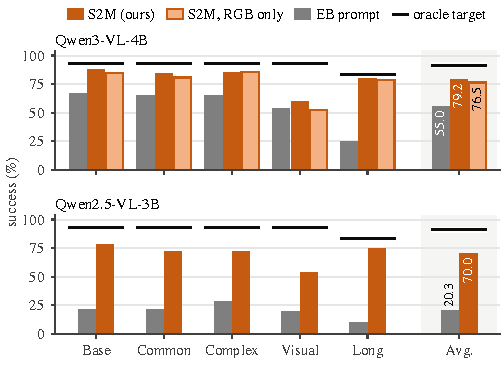
\includegraphics[width=0.7\linewidth]{figures/results.pdf}
\caption[Success with the same local model]{EB-Navigation test success with the same local model (60 episodes per
subset). Black line: geometric planner given the true target position (oracle target). The RGB-only configuration
was run with Qwen3-VL-4B.}
\label{fig:results}
\end{figure}

With Qwen3-VL-4B, \ours succeeds in \nSThree\% of the episodes against \nEBThree\% for the EB prompt, a paired gain of
\nGainThree{} percentage points (95\% CI [${+}\nGainThreeLo$, ${+}\nGainThreeHi$], $p\nGainThreeP$). Over three test
runs its average success ranges from \nSThreeMin\% to \nSThreeMax\% (standard deviation \nSThreeSD{} percentage
points), and the two RGB-only runs differ by a similar amount. Per episode, compared with the first run of \ours, the
EB prompt solves \nDiscThreeLosses{} episodes that \ours fails and fails \nDiscThreeWins{} that \ours solves; with
Qwen2.5-VL-3B the counts are \nDiscTwoLosses{} and \nDiscTwoWins. Every single run of \ours is significantly better
than the EB prompt (exact McNemar test, largest $p\nMcNThreeWorst$).
With Qwen2.5-VL-3B, \ours reaches \nSTwo\% against \nEBTwo\% (${+}\nGainTwo$\,pp, CI [${+}\nGainTwoLo$,
${+}\nGainTwoHi$]). \Cref{fig:subsets} shows the
success of every configuration on each subset, from the prompted agent to the oracle, and \cref{tab:ci} gives the
confidence interval of every configuration run on EB-Navigation and of the paired differences on which the
conclusions rest. Scaling the benchmark's agent tenfold within a model family buys \nScaleQwen{} percentage points
(Qwen2.5-VL, 7B to 72B) and \nScaleIntern{} (InternVL3, 8B to 78B); changing the role of a 4B model buys as much, and
closes \nGapClosed\% of the gap between the EB prompt and the oracle planner. The gain follows each of the four
predictions.

\begin{table}[htbp]
\centering\small
\caption[Confidence intervals of the EB-Navigation results]{EB-Navigation test success of the configurations run
in this thesis, and paired differences, with 95\% bootstrap confidence intervals and sign-flip permutation
$p$-values (\cref{sec:pre-protocol}).}
\label{tab:ci}
\begin{tabular*}{\linewidth}{@{\extracolsep{\fill}}llrcl@{}}
\toprule
Configuration & Model & Success (\%) & 95\% CI & \\
\midrule
EB prompt & Qwen3-VL-4B & \nEBThree & [\nEBThreeLo, \nEBThreeHi] & \\
Modular, single view & Qwen3-VL-4B & \nModThree & [\nModThreeLo, \nModThreeHi] & \\
\ours & Qwen3-VL-4B & \nSThree & [\nSThreeLo, \nSThreeHi] & \\
\ours, RGB only & Qwen3-VL-4B & \nRGBThree & [\nRGBThreeLo, \nRGBThreeHi] & \\
EB prompt & Qwen2.5-VL-3B & \nEBTwo & [\nEBTwoLo, \nEBTwoHi] & \\
\ours & Qwen2.5-VL-3B & \nSTwo & [\nSTwoLo, \nSTwoHi] & \\
Oracle target & true position & \nOracle & [\nOracleLo, \nOracleHi] & \\
\midrule
Paired difference & Model & $\Delta$ (pp) & 95\% CI & $p$\\
\midrule
\ours $-$ EB prompt & Qwen3-VL-4B & ${+}\nGainThree$ & [${+}\nGainThreeLo$, ${+}\nGainThreeHi$] & $\nGainThreeP$\\
\ours $-$ modular, single view & Qwen3-VL-4B & ${+}\nSOverMod$ & [${+}\nSOverModLo$, ${+}\nSOverModHi$] & $\nSOverModP$\\
Modular, single view $-$ EB prompt & Qwen3-VL-4B & ${+}\nModOverEB$ & [${+}\nModOverEBLo$, ${+}\nModOverEBHi$] & $\nModOverEBP$\\
\ours, RGB only $-$ EB prompt & Qwen3-VL-4B & ${+}\nGainRGB$ & [${+}\nGainRGBLo$, ${+}\nGainRGBHi$] & $\nGainRGBP$\\
\ours, RGB only $-$ \ours & Qwen3-VL-4B & $\nGapRGB$ & [$\nGapRGBLo$, ${+}\nGapRGBHi$] & $\nGapRGBP$\\
\ours $-$ EB prompt & Qwen2.5-VL-3B & ${+}\nGainTwo$ & [${+}\nGainTwoLo$, ${+}\nGainTwoHi$] & $\nGainTwoP$\\
Oracle $-$ \ours & Qwen3-VL-4B & ${+}\nGapOracle$ & [${+}\nGapOracleLo$, ${+}\nGapOracleHi$] & $\nGapOracleP$\\
\bottomrule
\end{tabular*}
\end{table}

\begin{figure}[htbp]
\centering
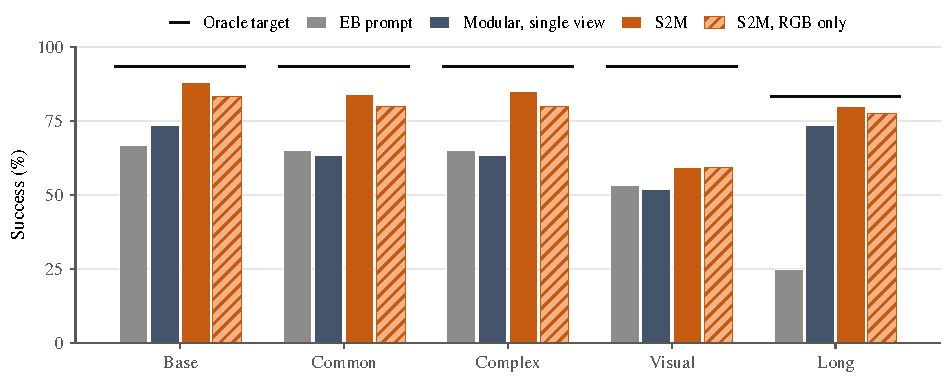
\includegraphics[width=\linewidth]{figures/th_subsets.pdf}
\caption[Success per subset]{EB-Navigation test success per subset with Qwen3-VL-4B, from the benchmark's agent to
the oracle (black line). \ours closes most of the gap to the oracle on every subset except Visual.}
\label{fig:subsets}
\end{figure}

\subsection{Prediction (i): the diagnosed failures collapse}
\Cref{fig:analysis}b breaks the failures down by outcome. Never-seen and blocked episodes fall by \nNeverRed{} and
\nBlockedRed\%, near misses by \nNearRed\%, and lost targets by \nLostRed\%. Per run, \ours never sees the target in \nNeverSThree{}
episodes (EB prompt: \nNeverEBThree), is blocked in \nBlockedSThree{} (\nBlockedEBThree), loses a seen target in
\nLostSThree{} (\nLostEBThree), and ends near it in \nNearSThree{} (\nNearEBThree). The look-around, the occupancy map,
and the memory remove the never-seen and blocked failures almost entirely and reduce the lost-after-seen ones, as
predicted. \Cref{tab:taxonomy,fig:outcomes} give the full taxonomy for both models. The change is the same
for both: the EB prompt spreads its failures over every category, while the failures of \ours collapse into
lost-after-seen and approach failures, most of which come from look-alikes (\cref{sec:exp-failures}).

\begin{figure}[htbp]
\centering
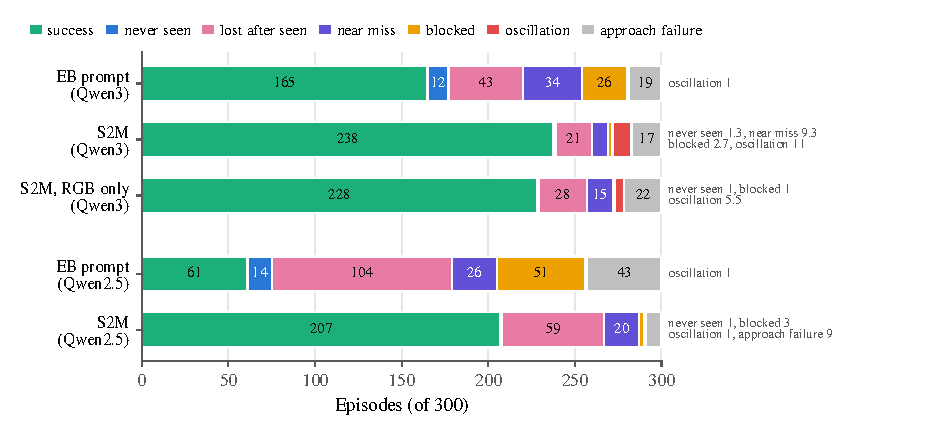
\includegraphics[width=\linewidth]{figures/th_outcomes.pdf}
\caption[Outcome of every episode]{Outcome of every EB-Navigation test episode by agent and model (first matching
rule of \cref{sec:pre-metrics}; mean over runs where a configuration was run repeatedly, so counts can be
fractional). Outcomes with fewer than 12 episodes are listed beside their bar.}
\label{fig:outcomes}
\end{figure}

\begin{figure}[htbp]
\centering
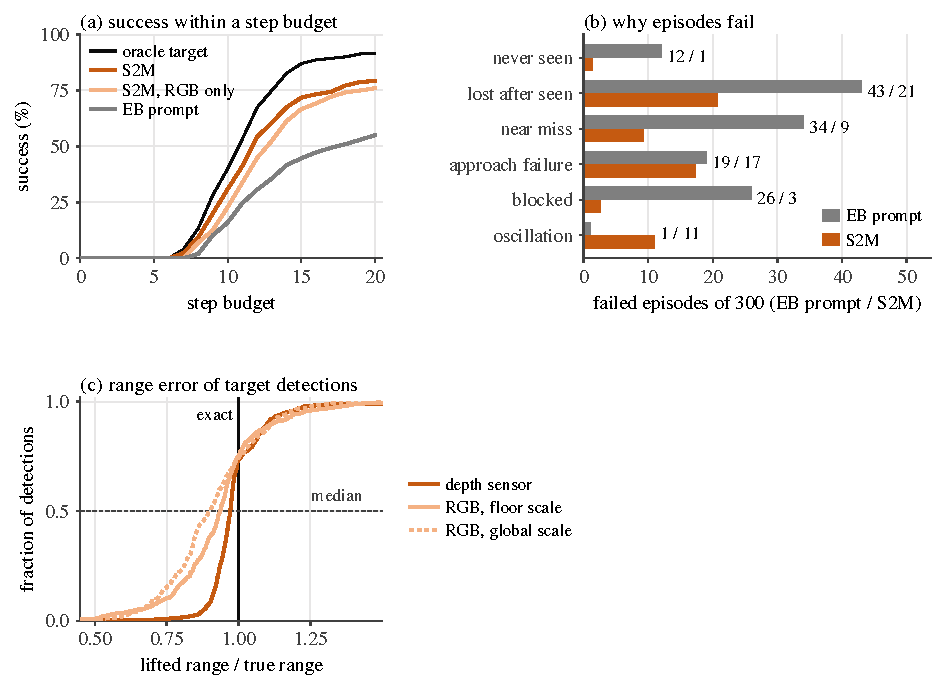
\includegraphics[width=\linewidth]{figures/analysis_thesis.pdf}
\caption[Step budget, failure outcomes, and range accuracy]{EB-Navigation test, Qwen3-VL-4B. \textbf{(a)}~Episodes
solved within a step budget, averaged over runs. \textbf{(b)}~Failed episodes by outcome (first matching rule,
\cref{sec:pre-metrics}; mean over the runs of \ours). \textbf{(c)}~Cumulative distribution of lifted over true range for
detections within 1\,m of the target (dashed: median), with the depth sensor and with monocular depth under a
per-frame floor scale (\cref{eq:floorscale}) or a global scale.}
\label{fig:analysis}
\end{figure}

\begin{table}[htbp]
\centering\small
\caption[Outcomes on EB-Navigation]{Outcomes on EB-Navigation test (episodes of 300; mean over runs where a
configuration was run repeatedly).}
\label{tab:taxonomy}
\begin{tabular*}{\linewidth}{@{\extracolsep{\fill}}lrrrrr@{}}
\toprule
& \multicolumn{3}{c}{Qwen3-VL-4B} & \multicolumn{2}{c}{Qwen2.5-VL-3B}\\
\cmidrule(lr){2-4}\cmidrule(l){5-6}
Outcome & EB prompt & \ours & \ours, RGB & EB prompt & \ours\\
\midrule
success & 165 & 237.7 & 228 & 61 & 207\\
never seen & 12 & 1.3 & 1 & 14 & 1\\
lost after seen & 43 & 20.7 & 28 & 104 & 59\\
near miss & 34 & 9.3 & 15 & 26 & 20\\
blocked & 26 & 2.7 & 1 & 51 & 3\\
oscillation & 1 & 11 & 5.5 & 1 & 1\\
approach failure & 19 & 17.3 & 21.5 & 43 & 9\\
\bottomrule
\end{tabular*}

\end{table}

\subsection{Prediction (ii): the largest gain on Long}
The gain is largest where the target starts behind the agent. On Long, \ours succeeds in \nSThreeLong\% against
\nEBThreeLong\%, only \nOracleGapLong{} percentage points below the oracle. On Base, Common, and Complex the gain is
$\nGainThreeBase$, $\nGainThreeCommon$, and $\nGainThreeComplex$ percentage points.

\subsection{Prediction (iii): the smallest gain on Visual}
On Visual the difference is not significant with Qwen3-VL-4B ($\nGainThreeVisual$\,pp, CI $[\nVisDiffLo, \nVisDiffHi]$,
$p\nVisDiffP$), and Visual is also the subset with the smallest gain with Qwen2.5-VL-3B ($\nGainTwoVisual$\,pp). This
is the subset on which single-view recognition was weakest (\cref{sec:diag-probe}); \cref{sec:exp-gap} examines it.

\subsection{Prediction (iv): far less dependence on model size}
Replacing Qwen3-VL-4B by Qwen2.5-VL-3B costs \ours \nScaleDrop{} percentage points and the EB prompt \nScaleDropEB{}
percentage points.
The smaller model loses much of its ability to plan in text, but its answers to per-image questions remain good
enough for the memory to use.
\IfFileExists{chapters/generated/qwen2b_text.tex}{The smallest model of the same family tests the prediction further. With Qwen3-VL-2B, \ours succeeds in \nSQTwo\% of the episodes and the EB prompt in \nEBQTwo\% (${+}\nGainQTwo$\,pp, CI [${+}\nGainQTwoLo$, ${+}\nGainQTwoHi$], $p\nGainQTwoP$). Halving the model from 4B to 2B costs \ours \nDropSQTwo{} percentage points and the EB prompt \nDropEBQTwo. From RGB alone, with the same monocular depth and dead reckoning as the 4B configuration, the 2B agent reaches \nRGBQTwo\%. The EB prompt with this model was run with the length-bounded output schema, which a development comparison chose over the official one, as for Qwen2.5-VL-3B (\cref{sec:pre-protocol}).
}{}

\section{Comparison with published agents}
\label{sec:exp-published}
\Cref{fig:landscape} places \ours among the agents of \cref{tab:main} by the size of their model. Even from RGB alone
(\nRGBThree\%), with a 4B model and no training, \ours exceeds every prompted MLLM up to GPT-4o,
\nNTrainFreeBelowRGB{} of the \nNTrainFree{} training-free agents, which build on GPT-4o and 8--32B
models~\cite{huang2025esca,wang2026mosaic,ju2026embodiskill,ma2026brainmem,lee2026emho,liang2026robofoundry}, and MuSix
and SVA, which train extra models around a 4B policy~\cite{jang2026musix,xie2026sva}. MuSix and SVA report episodes
36--60 and 37--60 of each subset, on which \ours (RGB only) reaches \nRGBMuSix{} and \nRGBSVA\%; EMHO reports its
best held-out score over search iterations on half of each subset. Only the tool-library
agents~\cite{zhou2026enabling} and RoboFoundry on GPT-6 Astra, which rewrites its prompts and code on the test
episodes, score higher. These comparisons use the results reported by the respective authors.

\begin{figure}[htbp]
\centering
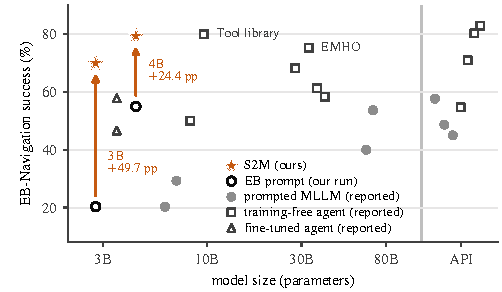
\includegraphics[width=0.7\linewidth]{figures/landscape.pdf}
\caption[Success against model size]{EB-Navigation success against model size (\cref{tab:main}). Arrows: gain of
\ours over the EB prompt with the same model; closed models share the API column.}
\label{fig:landscape}
\end{figure}

\section{Modularity alone is not enough}
\label{sec:exp-modular}
A modular structure removes the model from planning, but it does not by itself make the model's answers reliable.
The modular agent of \cref{sec:exp-setup} is \ours without multi-view fusion and the crop check: the same model,
map, planner, look-around, exploration, and exhaustion, acting on single-view detections. It reaches \nModThree\%, \nModOverEB{} percentage points above the EB prompt
($p\nModOverEBP$) but \nSOverMod{} below \ours (CI [${+}\nSOverModLo$, ${+}\nSOverModHi$], $p\nSOverModP$). Its gain
over the EB prompt falls almost entirely on Long ($\nModOverEBLong$\,pp), where the look-around alone finds the target;
on the other subsets it is level with the EB prompt. On Base, Common, and Complex, \ours exceeds the modular agent by $\nSOverModBase$,
$\nSOverModCommon$, and $\nSOverModComplex$ percentage points: these are the subsets in which the agent starts facing
the target and must hold on to it while approaching, which a single-view agent cannot do when the model places a
false box. Moving the state out of the model therefore gives part of the gain, and the evidence design for a
generative sensor gives the rest.

\section{Ablation of components}
\label{sec:exp-ablation}
\Cref{tab:abl} changes one element of \ours at a time and compares each variant with the full model over the same
episodes.

\begin{table}[t]
\centering\small
\setlength{\tabcolsep}{6pt}
\caption{Components and sensing on EB-Navigation test (Qwen3-VL-4B). $\Delta$: paired difference from the full model; $p$: sign-flip permutation test, Holm-corrected. Bold: significant.}
\label{tab:abl}
\resizebox{\linewidth}{!}{\begin{tabular}{@{}lrrrrrrrlr@{}}
\toprule
Variant & Base & Common & Complex & Visual & Long & Avg. & \multicolumn{2}{c}{$\Delta$ (95\% CI)} & $p$\\
\midrule
\ours (full) & 87.8 & 83.9 & 85.0 & 59.4 & 80.0 & 79.2 & \multicolumn{3}{c}{reference}\\
\midrule
\multicolumn{10}{@{}l}{\textit{Components}}\\
w/o fusion & 78.3 & 75.0 & 78.3 & 43.3 & 78.3 & 70.7 & $\mathbf{-8.6}$ & {\footnotesize[$-12.7$, $-4.6$]} & $3.4{\times}10^{-4}$\\
w/o look-around & 95.0 & 90.0 & 91.7 & 73.3 & 46.7 & 79.3 & $+0.1$ & {\footnotesize[$-4.2$, $+4.6$]} & $1.00$\\
w/o exhaustion & 86.7 & 81.7 & 85.0 & 58.3 & 76.7 & 77.7 & $-1.6$ & {\footnotesize[$-3.6$, $+0.3$]} & $0.38$\\
w/o crop check & 81.7 & 78.3 & 80.0 & 58.3 & 75.0 & 74.7 & $\mathbf{-4.6}$ & {\footnotesize[$-7.9$, $-1.3$]} & $0.04$\\
\midrule
\multicolumn{10}{@{}l}{\textit{Sensing}}\\
odometry noise (5\%, 2$^\circ$) & 90.0 & 88.3 & 88.3 & 60.0 & 81.7 & 81.7 & $+2.4$ & {\footnotesize[$-0.4$, $+5.4$]} & $0.38$\\
RGB only, global scale & 65.0 & 65.0 & 60.0 & 38.3 & 55.0 & 56.7 & $\mathbf{-22.6}$ & {\footnotesize[$-28.4$, $-16.8$]} & ${<}10^{-5}$\\
RGB only, floor scale & 83.3 & 80.0 & 80.0 & 59.2 & 77.5 & 76.0 & $-3.2$ & {\footnotesize[$-6.7$, $+0.2$]} & $0.31$\\
\bottomrule
\end{tabular}}
\end{table}


\Cref{fig:forest} shows the same differences with their confidence intervals. Two variants stand apart from the
rest: removing fusion and replacing the per-frame floor scale by a global one. The intervals of all other variants
include zero.

\begin{figure}[htbp]
\centering
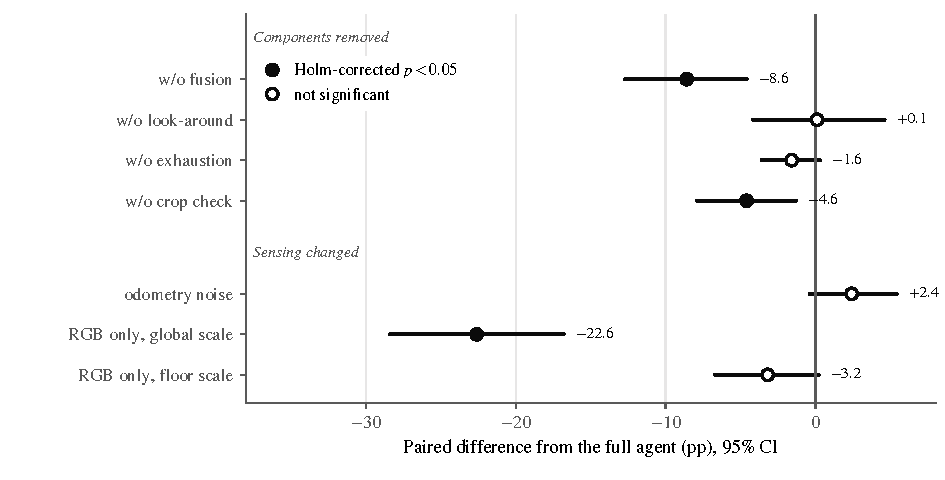
\includegraphics[width=\linewidth]{figures/th_forest.pdf}
\caption[Ablations with confidence intervals]{Paired difference in EB-Navigation success between each variant and
the full agent (Qwen3-VL-4B), with 95\% bootstrap intervals. Filled marker: significant after Holm correction ($p<0.05$); open marker: not
significant.}
\label{fig:forest}
\end{figure}

\subsection{Fusion keeps a found target}
Disabling multi-view fusion, so that each detection replaces the earlier hypotheses, lowers success by
\nAblFusionAbs{} percentage points (Holm $p\nAblFusionP$), the largest effect of any component. Fusion does not help the agent find the target: \nDetPrec\% of single lifted detections lie within
0.5\,m of it, and a hypothesis there reaches commitment in \nHoldNF{} episodes without fusion and \nHoldS{} with it.
Fusion keeps the target once found. Without it, each detection, including the false boxes of \cref{sec:diag-probe},
replaces the committed hypothesis, and lost targets rise from \nLostSThree{} to \nLostNF{} episodes and near misses
from \nNearSThree{} to \nNearNF.

\subsection{The look-around trades Long against the other subsets}
Removing the look-around leaves the average unchanged ($\nAblScan$\,pp) but changes Long by $\nAblScanLong$\,pp,
because the agent no longer turns to find a target behind it. The other subsets gain $\nAblScanOtherMin$ to
$\nAblScanOtherMax$\,pp, the steps that the turn no longer costs. On Long, \nScanLongFull{} episodes succeed only with
the look-around and \nScanLongAbl{} only without it (McNemar $p\nScanLongP$). The look-around is therefore what makes
the agent robust to where it starts. The inspection rule of \cref{sec:method-search} lowered this cost on the
development split, but on the test set the two sides still balance.

\subsection{The crop check and exhaustion}
Removing the crop check lowers success by \nAblZoomAbs{} percentage points (Holm $p\nAblZoomP$); it costs VLM calls,
not environment steps. Removing exhaustion changes success by $\nAblExhaust$\,pp (Holm $p\nAblExhaustP$). It acts only after the agent has
reached a look-alike: in \nExhVisLo--\nExhVisHi{} Visual episodes per run, where appearance-only goals produce
look-alikes that must be ruled out once visited, and in \nExhOtherLo--\nExhOtherHi{} on each other subset.

\section{One RGB camera is enough}
\label{sec:exp-sensing}
\label{sec:sensing}
\subsection{Pose}
Dead reckoning (\cref{eq:deadreckon}) is exact in heading and tilt. Its position error along the test trajectories,
caused by the simulator's grid snapping, averages \nDRmean\,m. Accumulated odometry noise of 5\% per translation and
2$^\circ$ per turn changes success by $\nAblOdom$ percentage points (\cref{tab:abl}).

\subsection{Depth}
Monocular depth with one global scale $\bar\sigma$ is not enough. With pose from the executed actions, \ours then
reaches \nRGBGlobal\%, level with the EB prompt ($\nGainGlobal$\,pp, $p\nDiscGlobalP$). The global scale places target
detections at a median \nRangeGlobal{} of their true range (\cref{fig:analysis}c) and lifts \nBlockGlobal\% of the
nearby floor above the obstacle threshold, so the agent walks to a point short of the target: \nShortGlobal{} failures
exhaust a hypothesis within 1\,m of it, none with the sensor. The per-frame floor scale (\cref{eq:floorscale}) lowers
the falsely blocked floor to \nBlockFloor\% and moves the range ratio to \nRangeFloor{} (sensor: \nRangeSensor).
Success rises to \nRGBThree\%, \nGainRGB{} percentage points above the EB prompt ($p\nGainRGBP$) and \nGapRGBAbs{}
below the depth sensor (Holm $p\nAblRgbfloorP$).

\section{Efficiency and cost}
\label{sec:exp-efficiency}
\ours also reaches the target in fewer steps. On the \nStepN{} episodes that both agents solve in every run, it needs
\nStepS{} steps against \nStepEB{} ($p\nStepP$). Within ten and fifteen steps it solves \nBudSTen{} and \nBudSFifteen\%
of the episodes against \nBudEBTen{} and \nBudEBFifteen\% for the EB prompt (\cref{fig:analysis}a).

The cost of an episode is spent differently. \ours makes \nCallsS{} VLM calls per episode against \nCallsEB{} for the
EB prompt, but each call asks one short question: it reads \nTokS{}k prompt tokens and generates \nTokSc{} tokens per
episode, against \nTokEB{}k and \nTokEBc{}k for the EB prompt, whose plans and reasoning dominate its generation.
Because generation is the slow part of decoding, many short questions are cheaper than a few long plans on a small
GPU. On the RTX 5060, which also renders the simulator, \ours takes \nSecS\,s per step and \tTimeEpS\,s per
episode on average, including rendering, all VLM calls, mapping, and planning, against \nSecEB\,s per step for the EB
prompt, \nSpeedUp{} times longer. The RGB-only configuration, which runs the depth network on the CPU, takes
\nSecRGB\,s per step. This is fast enough for a robot that moves 0.25\,m per step.

\section{Qualitative analysis}
\label{sec:exp-qualitative}
\Cref{fig:traj} shows three test episodes chosen by fixed rules, the first matching episode in index order of each
subset. In the Long episode (a), the EB prompt never turns toward the target, while \ours completes its look-around,
finds the target, and reaches it. In the Base episode (b), furniture blocks the EB prompt, which repeats rejected
moves; \ours plans around the obstacle on its map. In the Visual episode (c), \ours proposes only look-alikes and
fails while the EB prompt succeeds, an example of the recognition limit discussed next.

\begin{figure}[t]
\centering
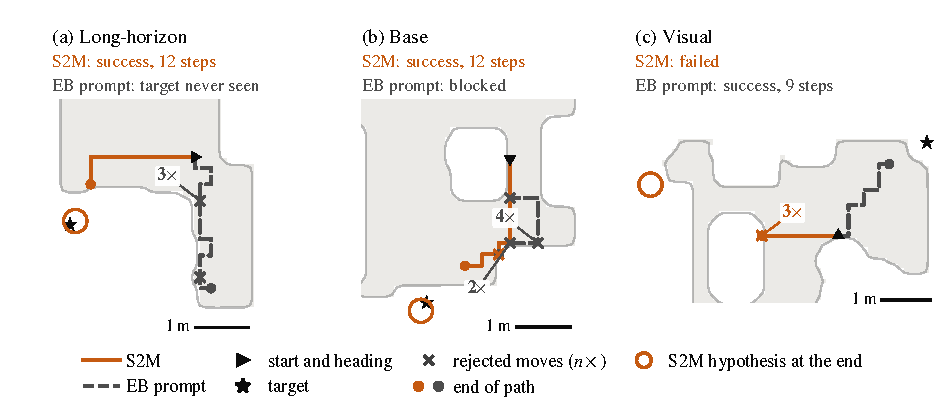
\includegraphics[width=\textwidth]{figures/trajectories_thesis.pdf}
\caption{Trajectories on three EB-Navigation test episodes (Qwen3-VL-4B) and the hypotheses of \ours at the end of each. Grey: reachable floor; targets on furniture lie outside it. $n\times$: rejected moves at one spot. (a)~the target starts behind the agent; (b)~furniture blocks the EB prompt; (c)~\ours proposes only look-alikes.}
\label{fig:traj}
\end{figure}


\Cref{fig:episode} looks inside one successful episode, the Long-horizon episode of \cref{fig:arch,tab:trace}. The
camera frames show what the VLM sees and where it places its box, and the plot below shows how the evidence of each
hypothesis develops. The agent turns away from an empty wall (step 0), sees the alarm clock and commits to it as
soon as it appears (step 2), keeps it while the model briefly boxes a look-alike (step 7), and reaches it with high
evidence (step 13). The look-alikes never approach the commit threshold.

\begin{figure}[htbp]
\centering
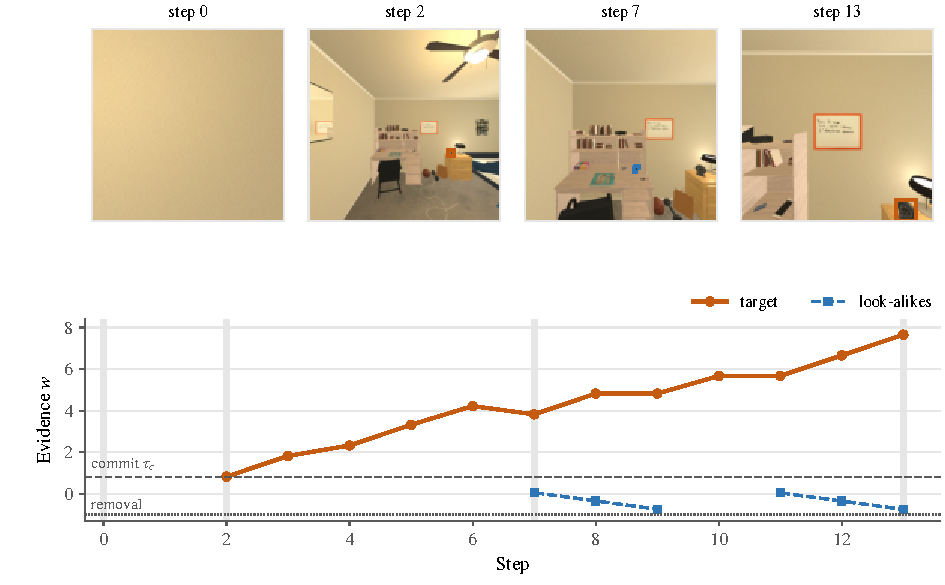
\includegraphics[width=\linewidth]{figures/th_episode.pdf}
\caption[Inside one episode]{Inside one Long-horizon test episode of \ours (Qwen3-VL-4B, target: alarm clock).
Top: camera frames at four steps, re-rendered from the saved trajectory, with the VLM's box (orange solid: on the
target; white: on a look-alike). Bottom: evidence of every hypothesis over the episode; grey bands and bold
step numbers mark the frames shown above. The episode ends in success after step 13, before either look-alike reaches
the removal line.}
\label{fig:episode}
\end{figure}

\section{The remaining failures of \ours}
\label{sec:exp-failures}
The failures that remain are of a different kind from those of the EB prompt. \Cref{tab:taxonomy} shows that \ours
almost never fails to see the target or gets blocked; its largest remaining category is \emph{lost after seen}, with
\tLostSAll{} episodes per run. Of these, \tLostSVisual{} fall on Visual, where the agent ``sees'' a look-alike that it
has proposed in place of the target and the true target is visible only in passing. Outside Visual, \ours loses a seen
target in a few episodes per subset. Near misses (\nNearSThree{} per run) and approach failures are also concentrated on Visual,
where the agent approaches a candidate that is not the target. With Qwen2.5-VL-3B, lost-after-seen is the largest failure mode for both agents, but \ours reduces it
from \nLostEBTwo{} to \nLostSTwo{} episodes.

\section{The remaining gap: appearance-only goals}
\label{sec:exp-gap}
Visual is the weakest subset in every run of \ours (\nVisSRLo--\nVisSRHi\%), accounts for \nVisGapShare\% of the gap to
the oracle, and is the only subset on which the gain over the EB prompt is not significant. The failure is recognition. A
candidate comes within 0.5\,m of the target in \nRecallOtherLo--\nRecallOtherHi\% of the episodes of every other subset
but in only \nRecallVisLo--\nRecallVisHi\% of the Visual ones, and \nVisFailNoCand{} of the \nVisFail{} Visual failures
never produce one. No memory can recover a target that the sensor never proposes; this limit lies in the model.

\section{RoboTHOR ObjectNav}
\label{sec:exp-robothor}
On the full RoboTHOR validation split, \ours reaches \nRoboSR\% success (CI [\nRoboSRLo, \nRoboSRHi]) and \nRoboSPL\%
SPL. \Cref{tab:robothor} compares it with published methods. Among zero-shot methods its success rate is below only
ForesightNav, which uses a 12B model~\cite{liu2026foresightnav}, and STRIVE, which uses Gemini-2.0-flash with a
detector~\cite{zhu2025strive}; its SPL is second only to STRIVE and above that of the ProcTHOR policy trained for the
task~\cite{deitke2022procthor}. Success ranges from \nRoboWorst\% (vases) to \nRoboBest\% (basketballs) by category
(\cref{fig:robothor}). \nRoboErr{} of the episodes end because the simulator rejects the start pose and are counted as
failures.

\subsection{How RoboTHOR episodes end}
RoboTHOR adds the decision to stop, so failures can come from stopping at the wrong place or from never stopping.
\Cref{fig:robothor-outcomes} separates the two. The agent issues Stop in \tRStop{} episodes, and \tRStopOk{} of these
succeed, a stop precision of \tRStopPrec\%. Of the \tRWrong{} wrong stops, \tRWrongNear{} end within 1.5\,m of the
target and the median one ends \tRWrongDist\,m away, so most wrong stops are at a look-alike rather than just short of
the target. In \tRLimit{} episodes the agent uses all 500 steps without stopping. In \tRLimitAppr{} of them it does
commit to and approach a candidate, but the stop check of \cref{sec:method-stop} rejects it (\tRLimitRej{} rejections
in total), so the agent exhausts the candidate and keeps searching; on average it spends \tRLimitExpl\% of these
episodes exploring. The stop check therefore trades wrong stops for unfinished episodes. Both failure types trace back to recognition: a look-alike that passes the stop check produces a wrong stop,
and a target that fails it produces an unfinished episode. With a model that tells targets from look-alikes more
reliably, the same agent would convert both into successes. Successful episodes take \tRStepsSucc{} steps at the median, and the agent runs at
\tRTimeStep\,s per step with \tRCallsEp{} VLM calls per episode.

\Cref{fig:robothor-budget} shows when the successes come and how the stop check decides. Success reaches
\tRBudHundred\% within 100 steps and \tRBudTwoHundred\% within 200, against \nRoboSR\% at the 500-step limit; nine in
ten successful episodes end within \tRStepsPninety{} steps. The last 300 steps therefore add only a few points: an
episode that has not found its target by then has usually committed to the wrong object or explored the wrong part of
the apartment. The stop check separates its two outcomes sharply: \tRCheckSure\% of its \tRCheckN{} presence answers lie below 0.1
or above 0.9, so the threshold of 0.5 is not a fine-tuned boundary.
The check rejects \tRRejN{} candidates in \tRRejEp{} episodes, and \tRRejEpOk{} of these episodes still succeed
after the agent moves on, which is the purpose of exhaustion on a benchmark that ends an episode only on Stop.

\begin{figure}[htbp]
\centering
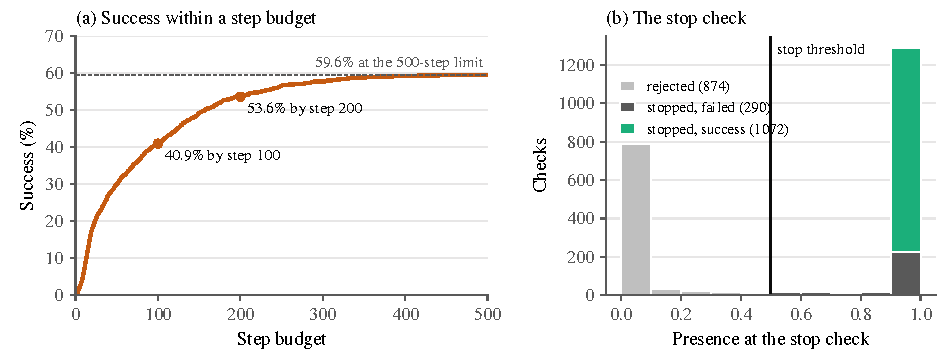
\includegraphics[width=\linewidth]{figures/th_robothor_budget.pdf}
\caption[RoboTHOR step budget and stop check]{RoboTHOR validation, \ours with Qwen3-VL-4B. \textbf{(a)}~Episodes
solved within a step budget, of all \nRoboN. \textbf{(b)}~Presence probability of the fresh query at every stop check,
by its outcome.}
\label{fig:robothor-budget}
\end{figure}

\begin{figure}[htbp]
\centering
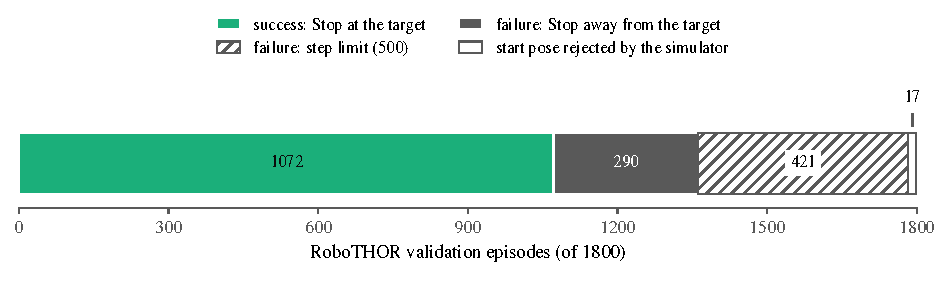
\includegraphics[width=\linewidth]{figures/th_robothor_outcomes.pdf}
\caption[How RoboTHOR episodes end]{How the \nRoboN{} RoboTHOR validation episodes of \ours end.}
\label{fig:robothor-outcomes}
\end{figure}

\begin{table}[!tb]
\centering\small
\caption{RoboTHOR ObjectNav validation (\nRoboN{} episodes), SR and SPL in \%. Bold: best; underlined: second.
$^\flat$As reported by SG-Nav~\cite{yin2024online}.}
\label{tab:robothor}
\begin{tabular*}{\linewidth}{@{\extracolsep{\fill}}llcrr@{}}
\toprule
Method & Input & Year & SR & SPL \\
\midrule
\multicolumn{5}{@{}l}{\textit{Zero-shot}}\\
CoW~\cite{gadre2022cows} & RGB-D & 2022 & 26.7 & 16.9 \\
LGX~\cite{dorbala2024lgx} & RGB-D & 2024 & 35.0 & 21.9 \\
ESC~\cite{zhou2023esc} & RGB-D & 2023 & 38.1 & 22.2 \\
L3MVN$^\flat$~\cite{yu2023l3mvn} & RGB-D & 2023 & 41.2 & 22.5 \\
VLFM$^\flat$~\cite{yokoyama2023vlfm} & RGB-D & 2023 & 42.3 & 23.0 \\
OpenFMNav$^\flat$~\cite{kuang2024openfmnav} & RGB-D & 2024 & 44.1 & 23.3 \\
SG-Nav~\cite{yin2024online} & RGB-D & 2024 & 47.5 & 24.0 \\
UniGoal~\cite{yin2025unigoal} & RGB-D & 2025 & 48.0 & 24.2 \\
CogNav~\cite{cao2024cognav} & RGB-D & 2024 & 54.6 & 24.3 \\
MVP-Nav~\cite{xie2026mvpnav} & RGB & 2026 & 57.5 & 26.8 \\
ForesightNav~\cite{liu2026foresightnav} & RGB-D & 2026 & 62.5 & 32.9 \\
STRIVE~\cite{zhu2025strive} & RGB-D & 2025 & \textbf{68.1} & \textbf{36.3} \\
\multicolumn{5}{@{}l}{\textit{Trained for the task}}\\
ProcTHOR~\cite{deitke2022procthor,gadre2022cows} & RGB & 2022 & \underline{66.4} & 27.4 \\
\midrule
\ours (Qwen3-VL-4B) & RGB-D & this work & \nRoboSR & \underline{\nRoboSPL} \\
\bottomrule
\end{tabular*}
\end{table}


\begin{figure}[htbp]
\centering
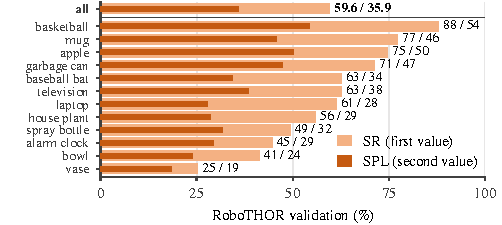
\includegraphics[width=0.7\linewidth]{figures/robothor_cats.pdf}
\caption{\ours on RoboTHOR validation by target category.}
\label{fig:robothor}
\end{figure}

\section{Summary}
The experiments confirm all four predictions of the diagnosis. With the same model, \ours gains as much as a tenfold
larger model gives the benchmark's agent, removes the never-seen and blocked failures and halves lost targets, gains
most on Long and least on Visual, and loses far less when the model shrinks. A modular agent with the same model recovers only part of the gain; multi-view fusion supplies most of the rest. The
agent works from RGB alone, uses fewer steps and \nSpeedUp{} times less time per step, and transfers to RoboTHOR. Its main remaining limit is the recognition
of objects described only by appearance.
